%%%%%%%%%%%%%%%%%%%%%%%%%%% asme2e.tex %%%%%%%%%%%%%%%%%%%%%%%%%%%%%%%
% Template for producing ASME-format articles using LaTeX            %
% Written by   Harry H. Cheng                                        %
%              Integration Engineering Laboratory                    %
%              Department of Mechanical and Aeronautical Engineering %
%              University of California                              %
%              Davis, CA 95616                                       %
%              Tel: (530) 752-5020 (office)                          %
%                   (530) 752-1028 (lab)                             %
%              Fax: (530) 752-4158                                   %
%              Email: hhcheng@ucdavis.edu                            %
%              WWW:   http://iel.ucdavis.edu/people/cheng.html       %
%              May 7, 1994                                           %
% Modified: February 16, 2001 by Harry H. Cheng                      %
% Modified: January  01, 2003 by Geoffrey R. Shiflett                %
% Use at your own risk, send complaints to /dev/null                 %
%%%%%%%%%%%%%%%%%%%%%%%%%%%%%%%%%%%%%%%%%%%%%%%%%%%%%%%%%%%%%%%%%%%%%%

%%% use twocolumn and 10pt options with the asme2e format
\documentclass[twocolumn,10pt,draft,cleanfoot]{asme2e}
\usepackage[]{epsfig,graphicx,epstopdf}
%% The class has several options
%  onecolumn/twocolumn - format for one or two columns per page
%  10pt/11pt/12pt - use 10, 11, or 12 point font
%  oneside/twoside - format for oneside/twosided printing
%  final/draft - format for final/draft copy
%  cleanfoot - take out copyright info in footer leave page number
%  cleanhead - take out the conference banner on the title page
%  titlepage/notitlepage - put in titlepage or leave out titlepage
%
%% The default is oneside, onecolumn, 10pt, final

%%% Replace here with information related to your conference
\confshortname{ASME/ISCIE 2012}
\conffullname{the ASME 2012 International Symposium On Flexible Automation}

%%%%% for date in a single month, use
\confdate{18-20}
\confmonth{June}
%%%%% for date across two months, use
%\confdate{August 30-September 2}
\confyear{2012}
\confcity{St. Louis, Missouri}
\confcountry{USA}

%%% Replace DETC2010/MECH-12345 with the number supplied to you
%%% by ASME for your paper.
\papernum{DETC2010/MECH-12345}

%%% You need to remove 'DRAFT: ' in the title for the final submitted version.
\title{Title goes here}

%%% first author
\author{Stephen Balakirsky\thanks{Address all correspondence to this author.}
    \affiliation{
	Intelligent Systems Division\\
	National Institute of Standards and Technology\\
	Gaithersburg, Maryland 20899\\
    Email: stephen.balakirsky@nist.gov
    }	
}

%%% second author
%%% remove the following entry for single author papers
%%% add more entries for additional authors
\author{Zeid Kootbally
    \affiliation{Department of Mechanical Engineering\\
	University of Maryland\\
	College Park, Maryland, 20742\\
	Email: zeid.kootbally@nist.gov
    }
}


\begin{document}

\maketitle

%%%%%%%%%%%%%%%%%%%%%%%%%%%%%%%%%%%%%%%%%%%%%%%%%%%%%%%%%%%%%%%%%%%%%%
\begin{abstract}
{\it Abstract goes here (less than 150 words).}
\end{abstract}
\section*{INTRODUCTION}
Robots have now become a part of many people's everyday lives. Whether as simple toys used by children, floor cleaning robots used in the home, or high precision industrial manipulators used in manufacturing, these systems are quickly changing the ways in which we play and work. One can no longer make the assumption that robots will exist in enclosed areas, or that the programmer or developer of the systems will be highly-skilled robotics experts. Indeed, new open source projects in robotic control systems such as the Robot Operating System (ROS)\footnote{Certain commercial software and tools are identified in this paper in order to explain our research. Such identification does not imply recommendation or endorsement by the authors, nor does it imply that the software tools identified are necessarily the best available for the purpose.}\cite{ROSWeb} allow anyone with a Linux computer to download and run some of the most advanced robotic algorithms that exist. If the users desire a deeper knowledge of how these algorithms work, there is even a free robotics course from Stanford that may be taken online.

One thing that many of these individuals are missing is robotic hardware. Simulators exist to fill this void and allow both experts and novices to experiment with robotic algorithms in a safe, low-cost environment. However, to truly provide valid simulation, the simulator must provide noise models for sensors and must be validated. One modern robotic simulator, know as the Unified System for Automation and Robot Simulation (USARSim) \cite{USARSimWeb}  provides such a simulation platform. This simulator has been used by the expert robotics community for several years and has played an important role in developing robotics applications. Its uses include rapid prototyping, debugging, and development of many tasks ranging from legged robots playing soccer \cite{ZARATTI.LNAI.2007} to urban search and rescue (USAR) \cite{CARPIN.LNAI.2006,WANG.WSC.2003}. In fact, a search for the keyword ``USARSim'' on Google Scholar returns over 700 articles that have referenced the simulation platform.

One reason for the simulation environment's popularity is that it enables researchers to focus on algorithm development without having to worry about the hardware aspects of the robots. Simulation can be an effective first step in the development and deployment of new algorithms and provides extensive testing opportunities without the risk of harming personnel or equipment. Major components of the robotic architecture (for example, advanced sensors) can be simulated and enable the developers to focus on the algorithms or components in which they are interested without the need to purchase expensive hardware. This can be useful when development teams are working in parallel or when experimenting with novel technological components that may not be fully implemented or available.

Simulation can also be used to provide access to environments that would normally not be available to the development team. Particular test scenarios can be run repeatedly, with the assurance that conditions are identical for each run. The environmental conditions, such as time of day, lighting, or weather, as well as the position and behavior of other entities in the world can be fully controlled. In terms of performance evaluation, it can truly provide an ``apples-to-apples" comparison of different software running on identical hardware platforms in identical environments. Another important feature of a robotic simulator is easy integration of different robotic platforms, different scenarios, different objects in the scene, as well
as support for multi-robot applications.

This paper examines a new interface that allows the ROS control framework to communicate directly with USARSim thus opening up sophisticated robot control and development to an entirely new audience. Novice robot developers can now work with world class algoirthms from the safety of their computer without the expense of actual robotic hardware.
This paper describes the interface connecting the USARSim framework with the ROS framework. The following sections describe, analyze and illustrate the new interface for the navigation of a mobile robot base, control of a robotic arm, and interface to existing sensors. In addition, a novel sensor interface is presented that allows the simulator to mimic a sensor processing system that produces the 6-degree-of-freedom pose for known objects.

%The rest of this paper is organized as follows: Section~\ref{s:background} gives an overview of USARSim and ROS. Section~\ref{s:topics} describes the specification of the topics addressed in ROS. Section~\ref{s:interface} details the interface and the associated commands to setup and run the interface. Section~\ref{s:navigation} displays examples of the interface running the navigation and motion stacks for mobile robots and robotic arms, respectively. Section~\ref{s:conclusion} concludes this paper and gives an overview of the future work. 
\section*{BACKGROUND}
In order to experiment with robotic systems, a researcher requires a controllable robotic platform, a control system that interfaces to the robotic system and provides behaviors for the robot to carry out, and an environment to operate in.  This paper examines an open source (the game engine is free, but license restrictions do apply), freely available framework capable of fulfilling all of these requirements. This framework is composed of the USARSim framework that provides the robotic platform and environment, and the ROS framework that provides the control system.

\subsection*{The USARSim Framework}
USARSim~\cite{CARPIN.LNAI.2006,WANG.WSC.2003} is a high-fidelity physics-based simulation system based on the Unreal Developers Kit (UDK)~\cite{UDKWeb} from Epic Games. USARSim was originally developed under a National Science Foundation grant to study Robot, Agent, Person Teams in Urban Search and Rescue~\cite{LEWIS.ICHC.2003}. Since that time, it has been turned into a NIST led community supported open source project that provides validated models of robots, sensors, and environments.

%Altogether, the Karma Physics engine~\cite{KarmEngine} and high-quality 3D rendering facilities of the Unreal game engine allow the creation of realistic simulation environments that provide the embodiment of a robotic system. Furthermore, USARSim comes with tools to develop objects and environments (Unreal Editor) and it is possible to control actors in the game through a TCP/IP socket API.

Through its usage of UDK, USARSim utilizes the physX phsyics engine~\cite{physXWeb} and high-quality 3D rendering facilities to create a realistic simulation environment that provides the embodiment of, and environment for a robotic
system. The current release of USARSim consists of various environmental models, models of commercial and experimental robots, and sensor models. High fidelity at low cost is made possible by building the simulation on top of a game engine. By loading the most
difficult aspects of simulation to a high volume commercial platform (available for free to most users) which provides superior visual rendering and physical modeling, full user effort can be devoted to the robotics-specific tasks of modeling platforms, control systems, sensors, interface tools and environments. These tasks are in turn accelerated by the advanced editing and development tools integrated with the game engine. This leads to a virtuous spiral in which a wide range of platforms can be modeled with greater fidelity in a short period of time.

USARSim was originally based upon simulated environments in the USAR domain. Realistic disaster scenarios as well as robot test methods were created (Figure~\ref{TestRoom}).
Since then, USARSim has been used worldwide and more environments have been developed for different purposes. Other environments such as the NIST campus (Figure~\ref{3D_World-b}) and factories (Figure~\ref{3D_World-c}) have been used to test the performance of algorithms in different efforts~\cite{WANG.HFES.2005,BALAGUER.IROS.2008,KOOTBALLY.ITEA.2010}. The simulation is also widely used for the RoboCup Virtual Robot Rescue Competition \cite{RoboCupWeb}, the IEEE Virtual Manufacturing and Automation Challenge \cite{VMACWeb} and has been applied to the DARPA Urban Challenge (Figure~\ref{3D_World-a}).

\begin{figure}[t!]
\centering
\subfigure[Test Room.]{\label{TestRoom}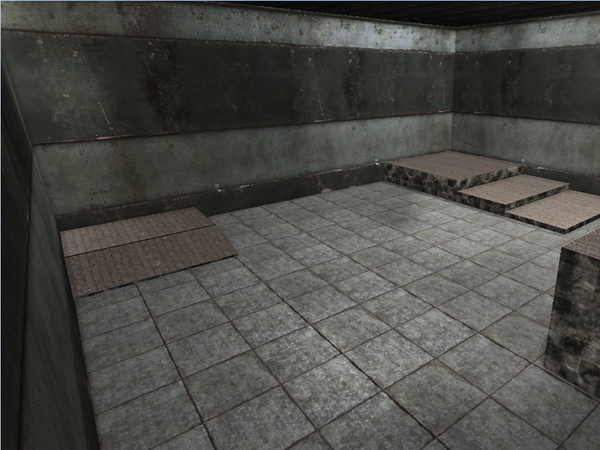
\includegraphics[width=4cm]{Figures/Worlds/testRoom.jpg}}\qquad
\subfigure[NIST main
campus.]{\label{3D_World-b}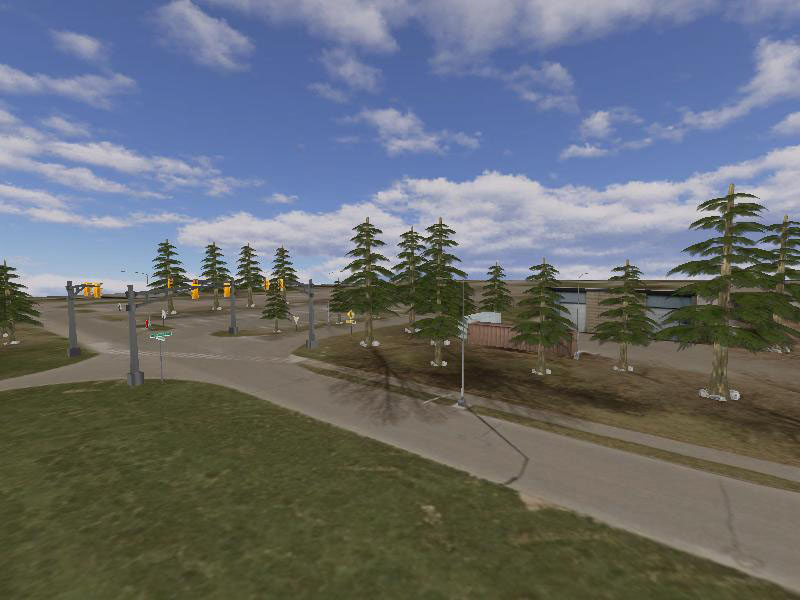
\psfig{file=Figures/Worlds/nist2.jpg,width=4cm}}\qquad
\subfigure[Factory,]{\label{3D_World-c}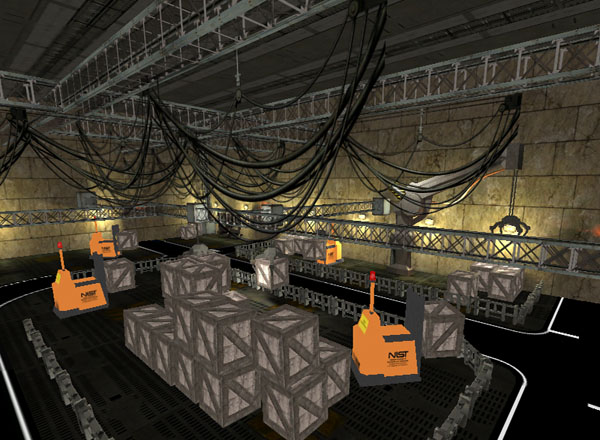
\psfig{file=Figures/Worlds/factory.jpg,width=4cm}}\qquad%
\subfigure[ARDA.]{\label{3D_World-a}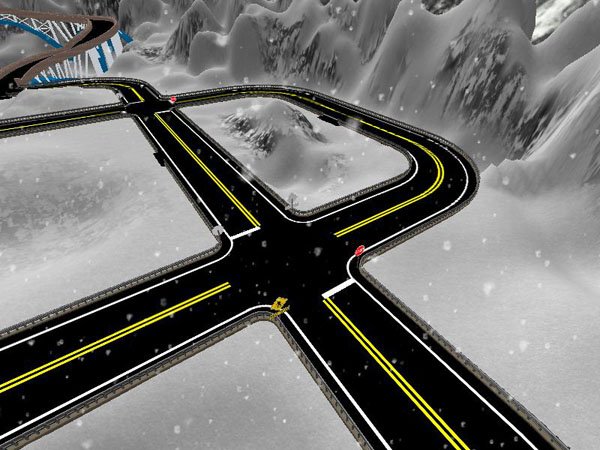
\psfig{file=Figures/Worlds/arda1.jpg,width=4cm}}
\caption{Sample of 3D environments in USARSim.} \label{3D_World}
\end{figure}

USARSim was initially developed with a focus on differential drive wheeled robots. However, USARSim's open source framework has encouraged wide community interest and support that now allows USARSim to offer multiple robots, including humanoid robots (Figure~\ref{Fig:Nao}), aerial platforms (Figure~\ref{Fig:AirRobot}), robotic arms (Figure~\ref{Fig:KR60}), and commercial vehicles (Figure~\ref{Fig:Kiva}). In USARSim, robots are based on physical computer aided design (CAD) models of the real
robots and are implemented by specialization of specific existing classes. This structure allows for easier development of new platforms that model custom designs.

All robots in USARSim have a chassis, and may contain multiple wheels, sensors and
actuators. The robots are configurable (specify types of
sensors/end effectors for example) through a configuration file that is read at runtime. The properties of the robots can
also be configured, such as the battery life and the frequency of
data transmission.

\begin{figure}[t!]
\centering
\subfigure[Aldebaran Robotics Nao.]{\label{Fig:Nao}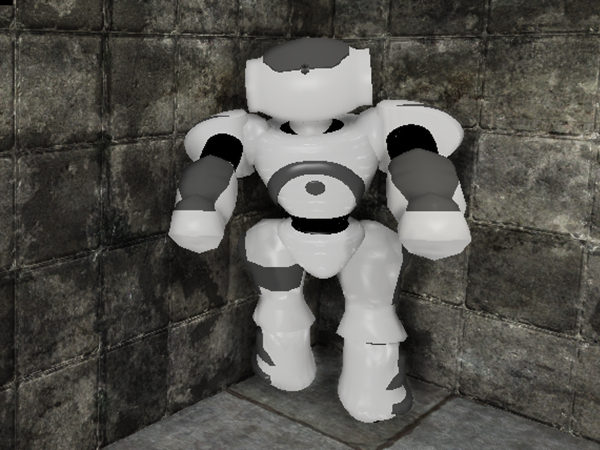
\includegraphics[width=4cm]{Figures/Robots/nao.jpg}}\qquad
\subfigure[Air Robot AR100B.]{\label{Fig:AirRobot}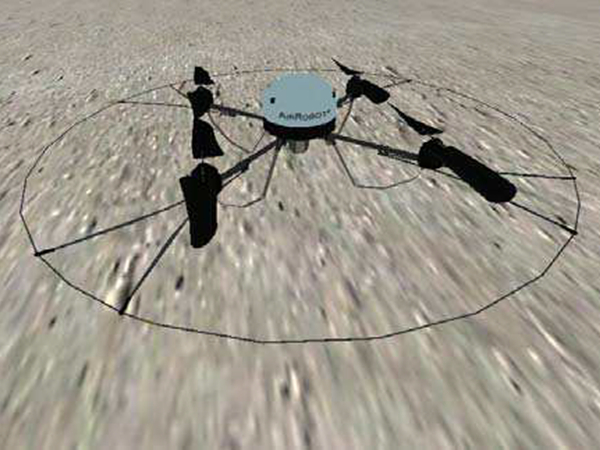
\includegraphics[width=4cm]{Figures/Robots/airRobot_2.jpg}}\qquad
\subfigure[Kuka KR60,]{\label{Fig:KR60}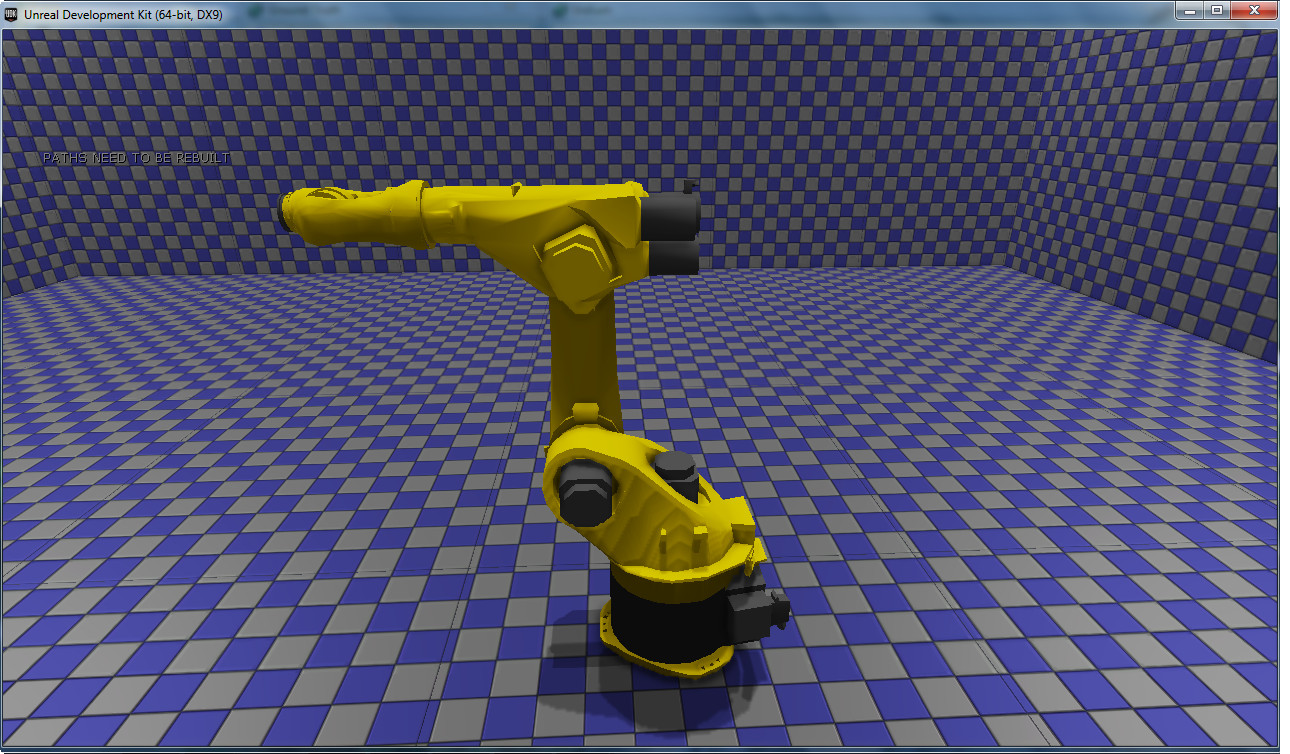
\includegraphics[width=4cm]{Figures/Robots/kr60.jpg}}\qquad
\subfigure[Kiva Robot.]{\label{Fig:Kiva}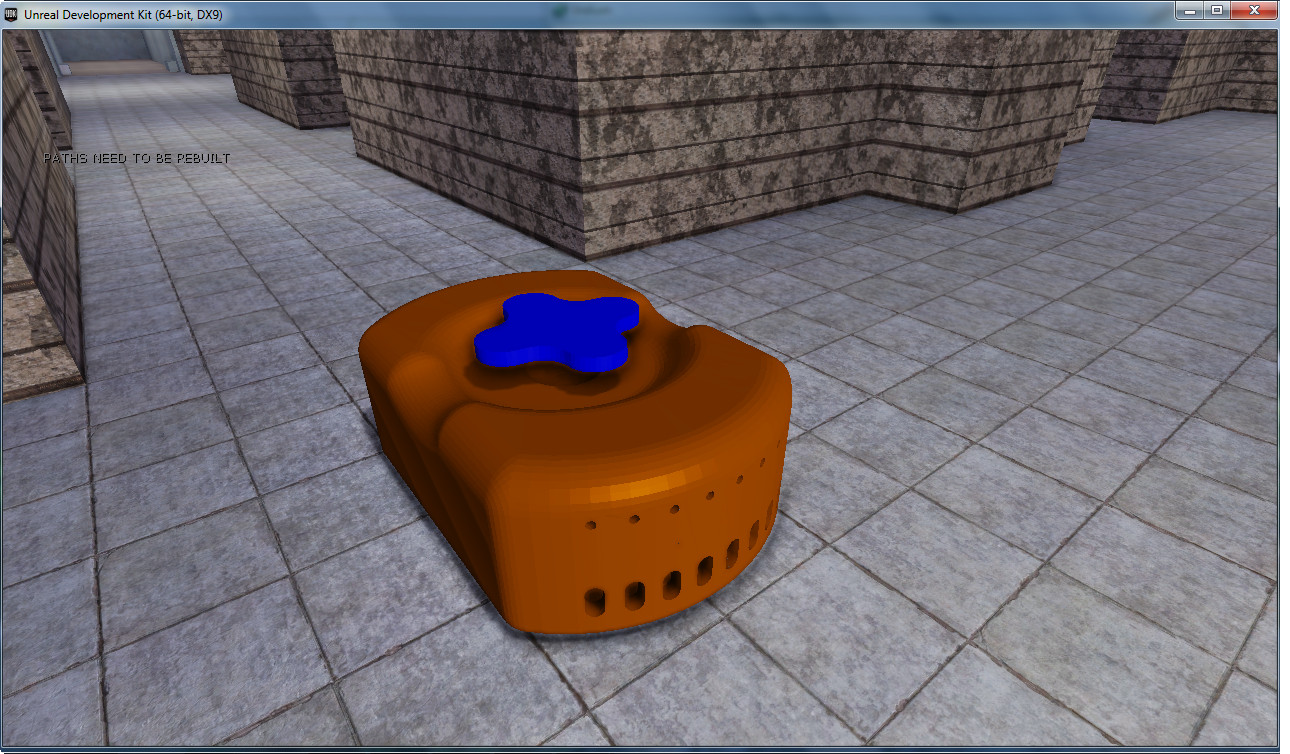
\includegraphics[width=4cm]{Figures/Robots/kiva.jpg}}
\caption{Sample of vehicles in USARSim.}
\end{figure}

\subsection*{The ROS Framework}

ROS is an open source framework designed to provide an abstraction layer to complex robotic hardware and software configurations. ROS delivers libraries and tools to help software developers create robot applications. ROS has been used in many robotic applications such as the Willow Garage's Personal Robots Program~\cite{WYOBEK.ICRA.2008} and the Stanford University STAIR project~\cite{QUIGLEY.AAAI.2007}.

ROS possesses a large range of tools and services that both users and developers alike can benefit from. The philosophical goals of ROS include an advanced set of criteria and can be summarized as: peer-to-peer, tools-based, multi-lingual, thin, and free and open source~\cite{QUIGLEY.ICRA.2009}. Furthermore, debugging at all levels of the software is made possible with the full source code of ROS being publicly available. Thus, the main developers of a project could benefit from the community and vice-versa.

\subsubsection*{Nomenclature}

ROS uses the concept of nodes, messages, topics, services, stacks, and packages. These terms are used throughout the rest of the paper and are detailed below~\cite{QUIGLEY.ICRA.2009}.
\begin{itemize}
\item[-] Node: A process that performs computation. Nodes communicate with each other by passing messages.
\item[-] Message: A strictly typed data structure. A node sends a message by publishing it to a given topic.
\item[-] Topic: A communication channel between two or more
nodes. A node that is interested in a certain kind of data will subscribe
to the appropriate topic. There may be multiple concurrent
publishers and subscribers for a single topic, and a single
node may publish and/or subscribe to multiple topics.
\item[-] Service: A remote procedure call defined by a string name and a pair
of strictly typed messages: one for the request and one for
the response.
\item[-] Package: A compilation of nodes that can easily be compiled and ported to other computers. Packages are necessary to build a complete ROS-based robot control system.
\item[-] Stack: Packages in ROS are organized into ROS stacks which simplifies the process of code sharing. 

\end{itemize} 
\section*{THE ROS/USARSIM INTERFACE}\label{s:interface}
Steve

Talk about the interface. RosSim node, topics, etc.
\subsection*{Sensor Interface}
Steve
\subsection*{Mobile Robot Control with The ROS Navigation Stack}
Control of mobile robots through the ROS/USARim interface is performed with the ROS navigation stack\footnote{http://www.ros.org/wiki/navigation}. The navigation stack is a 2D navigation stack that takes in information from odometry, sensor streams, and a goal pose and outputs safe velocity commands that are sent to a mobile base. The velocity commands are sent it the form of: x velocity, y velocity, theta velocity. Better performance of the navigation stack can be achieved by meeting the following requirements:
\begin{itemize}
\item[-] The robot has to use either differential drive or holonomic drive.
\item[-] A planar laser has the be mounted on the mobile base. This laser is used for map building and localization.
\item[-] The performance of the navigation stack will be best on robots that are nearly square or circular. It does work on robots of arbitrary shapes and sizes, but it may have difficulty with large rectangular robots in narrow spaces like doorways.
\end{itemize}

Although different models of mobile robot are developed in USARSim, the Pioneer 3-AT (P3AT) (Figure~\ref{fig:p3at}) appears to be a suitable candidate to use the navigation stack. The P3AT is a small square-shaped differential wheeled robot with a SICK Laser Measurement Sensor (LMS) 200 mounted on his base. The P3AT is also widely employed for research and prototyping applications involving mapping, navigation, monitoring, reconnaissance, vision, manipulation, cooperation, and other behaviors.

\begin{figure}[t!]
\centering
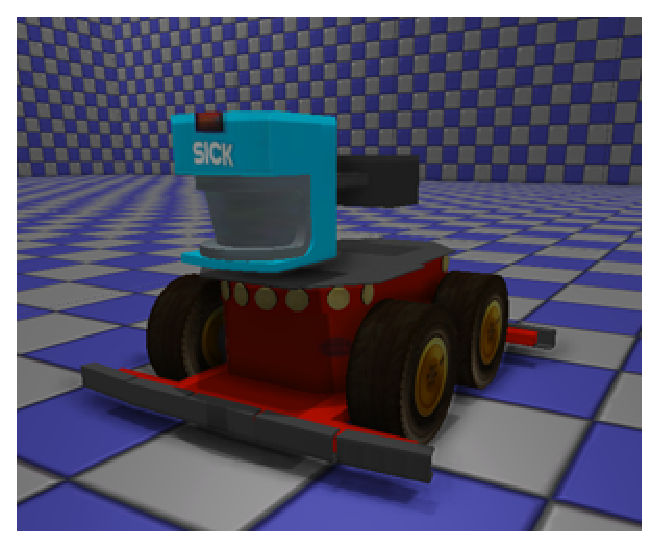
\includegraphics[width=4cm]{Figures/Robots/P3AT.eps}
\caption{Pioneer 3-AT (P3AT) in USARSim.}\label{fig:p3at}
\end{figure}




\subsubsection*{Low-level Navigation}
The ROS/USARSim interface allows the startup and the control of the default P3AT base controllers by directly sending velocity commands to the base. This task was performed using the following commands:
\begin{enumerate}
\item Bring up an environment in USARSim
\item \$ \texttt{roscore}
\item \$ \texttt{roslaunch usarsim usarsim.launch}
\item \$ \texttt{rosrun teleop\_twist\_keyboard teleop\_twist\_keyboard.py}
\end{enumerate}

In the first step, the user starts the environment in USARSim. If an environment is not up and running, passing messages between ROS and USARSim is not possible. The second step starts \texttt{roscore}, a collection of nodes and programs that are a pre-requisites of a ROS-based system. \texttt{roscore} must run in order for ROS nodes to communicate. The third step launches the \texttt{usarsim.launch} file. This launch file contains information necessary to connect ROS to the computer running the server (USARSim), to set up the appropriate robot (the P3AT in this case) at the correct location in the environment, to launch the proper ROS topics and to start the \texttt{RosSim} node. The last step starts the \texttt{teleop\_twist\_keyboard} node which sends velocity commands to the \texttt{RosSim} node through the computer keyboard. At this point, the P3AT can be controlled by keyboard teleop in the USARSim environment.

Figure~\ref{fig:teleop} illustrates the communication between the \texttt{RosSim} and the \texttt{teleop\_twist\_keyboard} nodes (in ovals). The keyboard inputs are converted in velocity commands and then communicated to the \texttt{RosSim} node on the topic \texttt{cmd\_vel}. \texttt{RosSim} publishes two topics for the odometry (\texttt{GndTruth} and \texttt{InsTest}), one topic to keep track of multiple coordinate frames over time \texttt{tf}, and a topic for the laser scanner (\texttt{lms200}).
\begin{figure}[h!]
\centering
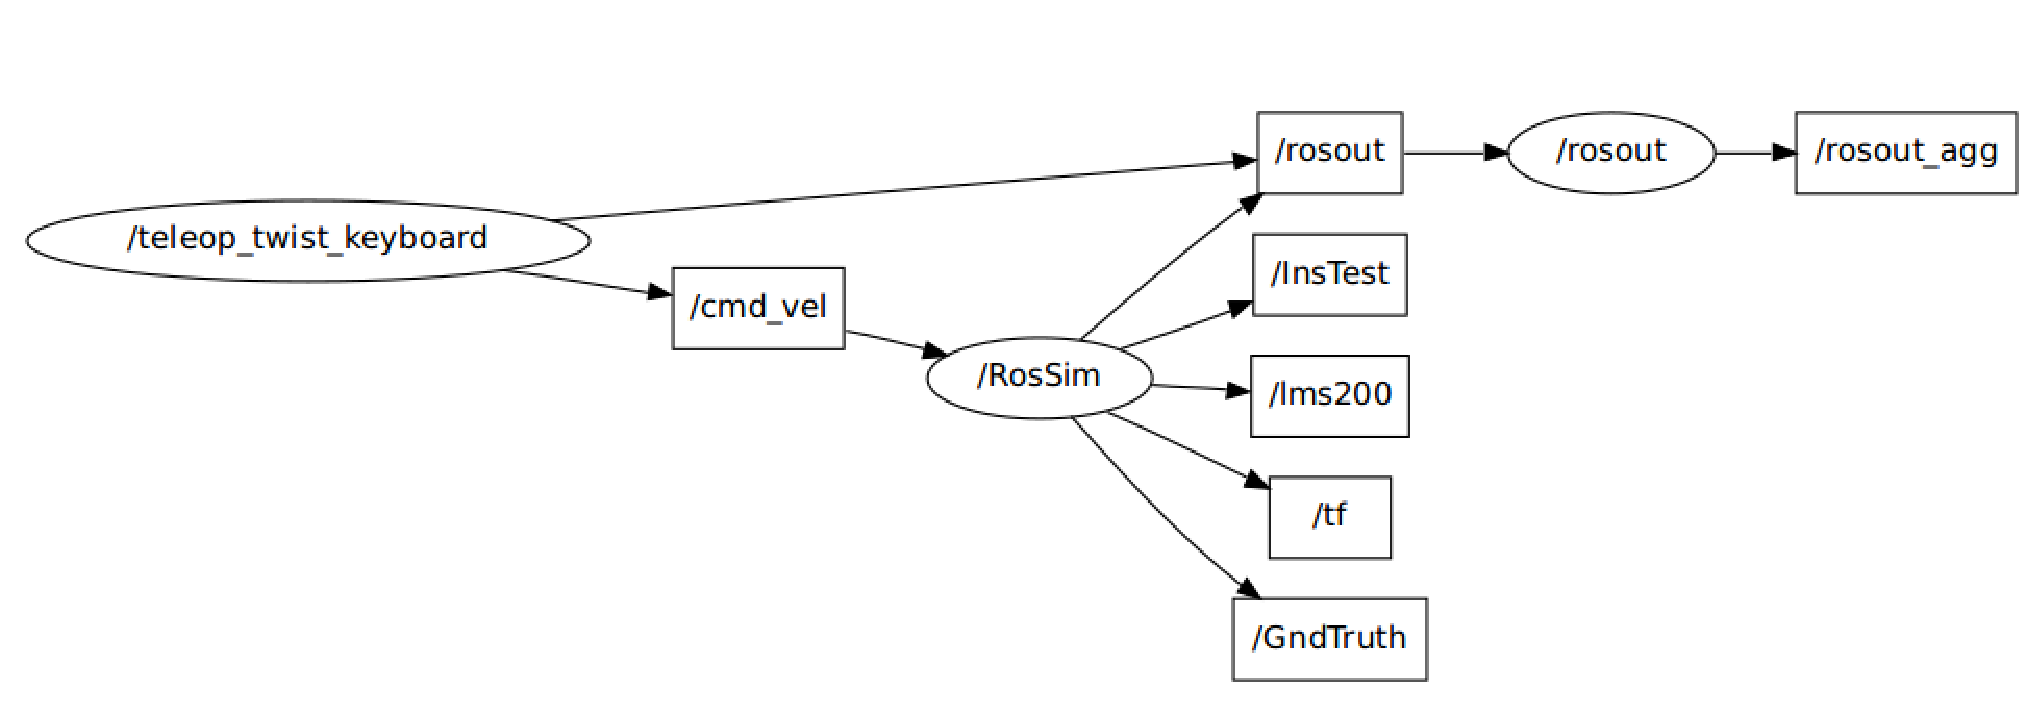
\includegraphics[width=9cm]{Figures/Misc/teleop-rossim-non-quiet.eps}
\caption{Mobile robot control at the lower level.}\label{fig:teleop}
\end{figure}

\subsubsection*{High-level Navigation}
This section describes how goals are sent using code to the P3AT to move to a particular location. Navigation at hight level is possible with the action specification for \texttt{move\_base}. This package provides an implementation of an action (\texttt{actionlib}) that, given a goal in the world, will attempt to reach it with a mobile base. The \texttt{move\_base} node links together a global and local planner to accomplish its global navigation task. 

\begin{figure}[h!]
\centering
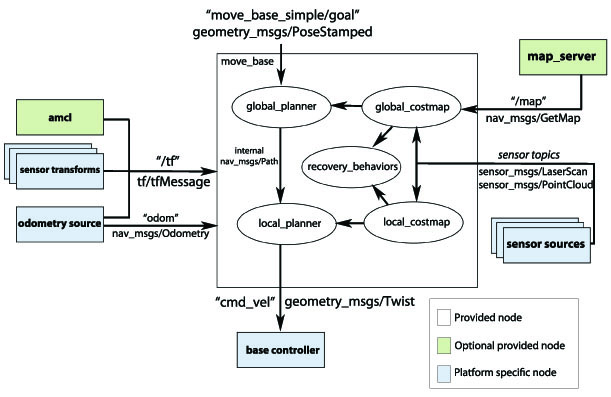
\includegraphics[width=9cm]{Figures/Misc/Navigation_Stack.eps}
\caption{Navigation stack setup.}\label{fig:navigation_stack}
\end{figure}
The \texttt{move\_base} node provides a ROS interface for configuring, running, and interacting with the navigation stack on a robot. The diagram in Figure~\ref{fig:navigation_stack} depicts a high-level view of the \texttt{move\_base} node and its interaction with other components of the navigation stack. The white components are required components that are already implemented, the green components are optional components that are already implemented, and the blue components must be created for each robot platform. 
%The blue components were created for the P3AT, enabling ROS to control the robot at lower and higher levels of the navigation stack.

 Before running the \texttt{move\_base} node on the P3AT, localization, mapping and navigation information were gathered in the \texttt{move\_base.launch} file.

Localization uses map, laser data, and odometry to situate the robot in relation to the environment. The \texttt{amcl} and the \texttt{map\_server} nodes are necessary for robot localization. \texttt{amcl} is a probabilistic localization system for a robot moving in 2D and implements the KLD-sampling\cite{DIETER.IJRS.2003}. The \texttt{amcl} node is launched from the
examples directory of the amcl package.

The \texttt{map\_server} uses an a priori map generated by the \texttt{map\_saver} command-line utility. The generated map is stored in pair of files. The YAML file describes the map metadata and references the image file. The image file encodes the occupancy data. 



\subsection*{Robotic Arm Interface}
Steve

\section*{SETUP AND RUN THE INTERFACE}\label{s:interface}

\section*{CONCLUSION AND FUTURE WORK}\label{s:conclusion}


%%%%%%%%%%%%%%%%%%%%%%%%%%%%%%%%%%%%%%%%%%%%%%%%%%%%%%%%%%%%%%%%%%%%%%
% The bibliography is stored in an external database file
% in the BibTeX format (file_name.bib).  The bibliography is
% created by the following command and it will appear in this
% position in the document. You may, of course, create your
% own bibliography by using thebibliography environment as in
%
% \begin{thebibliography}{12}
% ...
% \bibitem{itemreference} D. E. Knudsen.
% {\em 1966 World Bnus Almanac.}
% {Permafrost Press, Novosibirsk.}
% ...
% \end{thebibliography}

% Here's where you specify the bibliography database file.
% The full file name of the bibliography database for this
% article is asme2e.bib. The name for your database is up
% to you.
\bibliographystyle{asmems4}
\bibliography{PMAS-asme}



\end{document}
